\lstdefinestyle{mystyle}{
    basicstyle=\footnotesize,                
   	captionpos=b,            
   	tabsize=2
}
\lstset{style=mystyle}
%versi 2 (8-10-2016)
\chapter{Landasan Teori}
\label{chap:teori}
Bab ini akan membahas teori-teori yang akan menjadi dasar dari penelitian ini. Teori yang dibahas yaitu mengenai {\it Javadoc}, {\it Doclet} dan \LaTeX .

\section{Javadoc}
\label{sec:javadoc} 
{\it Javadoc} adalah sebuah perangkat lunak yang dimiliki oleh {\it Java} yang berguna untuk mengambil informasi dari sebuah komentar yang terdapat pada sekumpulan {\it source file Java} menjadi sebuah dokumentasi. Umumnya {\it Javadoc} menghasilkan sekumpulan {\it file} HTML yang mendeskripsikan sebuah kelas, {\it interface}, {\it method} dan {\it custom tag}. {\it Javadoc} dapat mengambil informasi tersebut dari sebuah {\it package Java}, sebuah {\it file Java} atau keduanya~\cite{javadoc:01:javadoc}.

\subsection{\textit{Processing of source files}}
\label{sec:javadoc}
{\it Javadoc} akan memproses {\it file} yang memiliki akhiran {\it ".java"}. {\it Javadoc} dapat mengambil informasi dari lebih dari 1 {\it file Java} atau sebuah {\it package}.

{\it Javadoc} secara otomatis akan menambahkan sebuah tautan yang mengarahkan ke sebuah {\it package}, kelas dan anggota dari kelas tersebut yang akan didokumentasikan pada saat {\it Javadoc} memprosesnya. Tautan tersebut berada pada beberapa posisi seperti:
\begin{enumerate}
	\item {\it Declaration} ({\it return types}, {\it argument types}, {\it field types}).
	\item {\it "See Also"} yang dihasilkan oleh {\it tag @see}.
	\item {\it In-line text} yang dihasilkan oleh {\it tag {@link}}.
	\item {\it Exception} yang dihasilkan oleh {\it tag @throws}.
	\item {\it Link "Specified by"} untuk {\it member} dari sebuah {\it interface}.
	\item {\it Link "Override"} untuk {\it member} dari sebuah kelas.
	\item Ringkasan daftar tabel {\it package}, kelas dan seluruh anggota dari kelas.
	\item Turunan dari setiap {\it package} dan kelas.
	\item Indeks.
\end{enumerate}

Dalam mengambil informasi yang terdapat dalam sebuah {\it package Java} atau beberapa {\it file Java} umumnya menghasilkan sebuah dokumentasi standar yang berbentuk {\it file} HTML dan format penulisan yang mengikuti standar {\it Javadoc}. Akan tetapi untuk menghasilkan sebuah format dokumentasi yang diinginkan, dapat mengimplementasi sebuah API yang disediakan oleh {\it Javadoc}.

\subsection{Terminologi}
\label{sec:terminologi}
Terdapat beberapa istilah yang memiliki arti spesifik dalam konteks {\it Javadoc} sebagai berikut:
\begin{itemize}
	\item {\it Generated Document}\\
	Dokumen yang dihasilkan oleh {\it Javadoc} adalah sebuah {\it file} HTML.
	\item {\it Name}\\
	Nama dari elemen program yang dideklarasikan atau dilakukan pemanggilan maka dapat berupa informasi lengkapnya seperti {\tt java.lang.String} dan {\tt java.lang.String.equals(java.lang.Object)} atau informasi pendeknya seperti {\tt String} dan {\tt equals(Object)}. Nama-nama tersebut dapat berupa nama {\it package}, kelas, {\it interface}, {\it field}, {\it constructor} atau {\it method}.
	\item {\it Documented Classes}\\
	Detail dari sebuah kelas dan {\it interface} akan didokumentasikan pada saat {\it Javadoc} berjalan. Untuk dapat didokumentasikan, {\it source file} harus tersedia, kemudian nama dari {\it source file} atau nama dari {\it package} tersebut harus diletakkan pada {\it Javadoc command-line}.
	\item {\it Included Classes}\\
	Kelas dan {\it Interface} akan didokumentasikan pada saat {\it Javadoc} berjalan, hal ini sama seperti {\it Documented Classes}.
	\item {\it Excluded Classes}\\
	Kelas dan {\it Interface} tidak akan didokumenasikan pada saat {\it Javadoc} berjalan.
	\item {\it Referenced Classes}\\
	Kelas dan {\it Interface} yang secara eksplisit disebutkan oleh kelas dan {\it interface} lainnya, seperti {\it return type}, {\it parameter type}, {\it cast type}, {\it extended class}, {\it implemented interface}, {\it imported class}, kelas yang digunakan pada {\it method body}, {\it @see}, {\it {@link}}, {\it {@linkplain}} dan {\it {@inheritDoc} tag}.
	%\item {\it External Referenced Classes}\\
	%Kelas yang tidak dihasilkan saat {\it Javadoc} berjalan. Dengan kata lain, kelas tersebut tidak diletakkan pada {\it Javadoc command-line}. {\it Links} akan dihasilkan jika sebuah kelas mengatakan memiliki {\it external references} atau {\it external link}.
\end{itemize}

\subsection{\textit{Source Files}}
\label{sec:source-files}
{\it Javadoc} akan menghasilkan {\it output} yang berasal dari 4 tipe {\it file}, yaitu sebagai berikut:
\begin{itemize}
	\item {\it Class Source Code Files}\\
	Setiap kelas atau {\it interface} memiliki dokumentasinya masing-masing.
	\begin{figure}[H]
	  \centering  
	  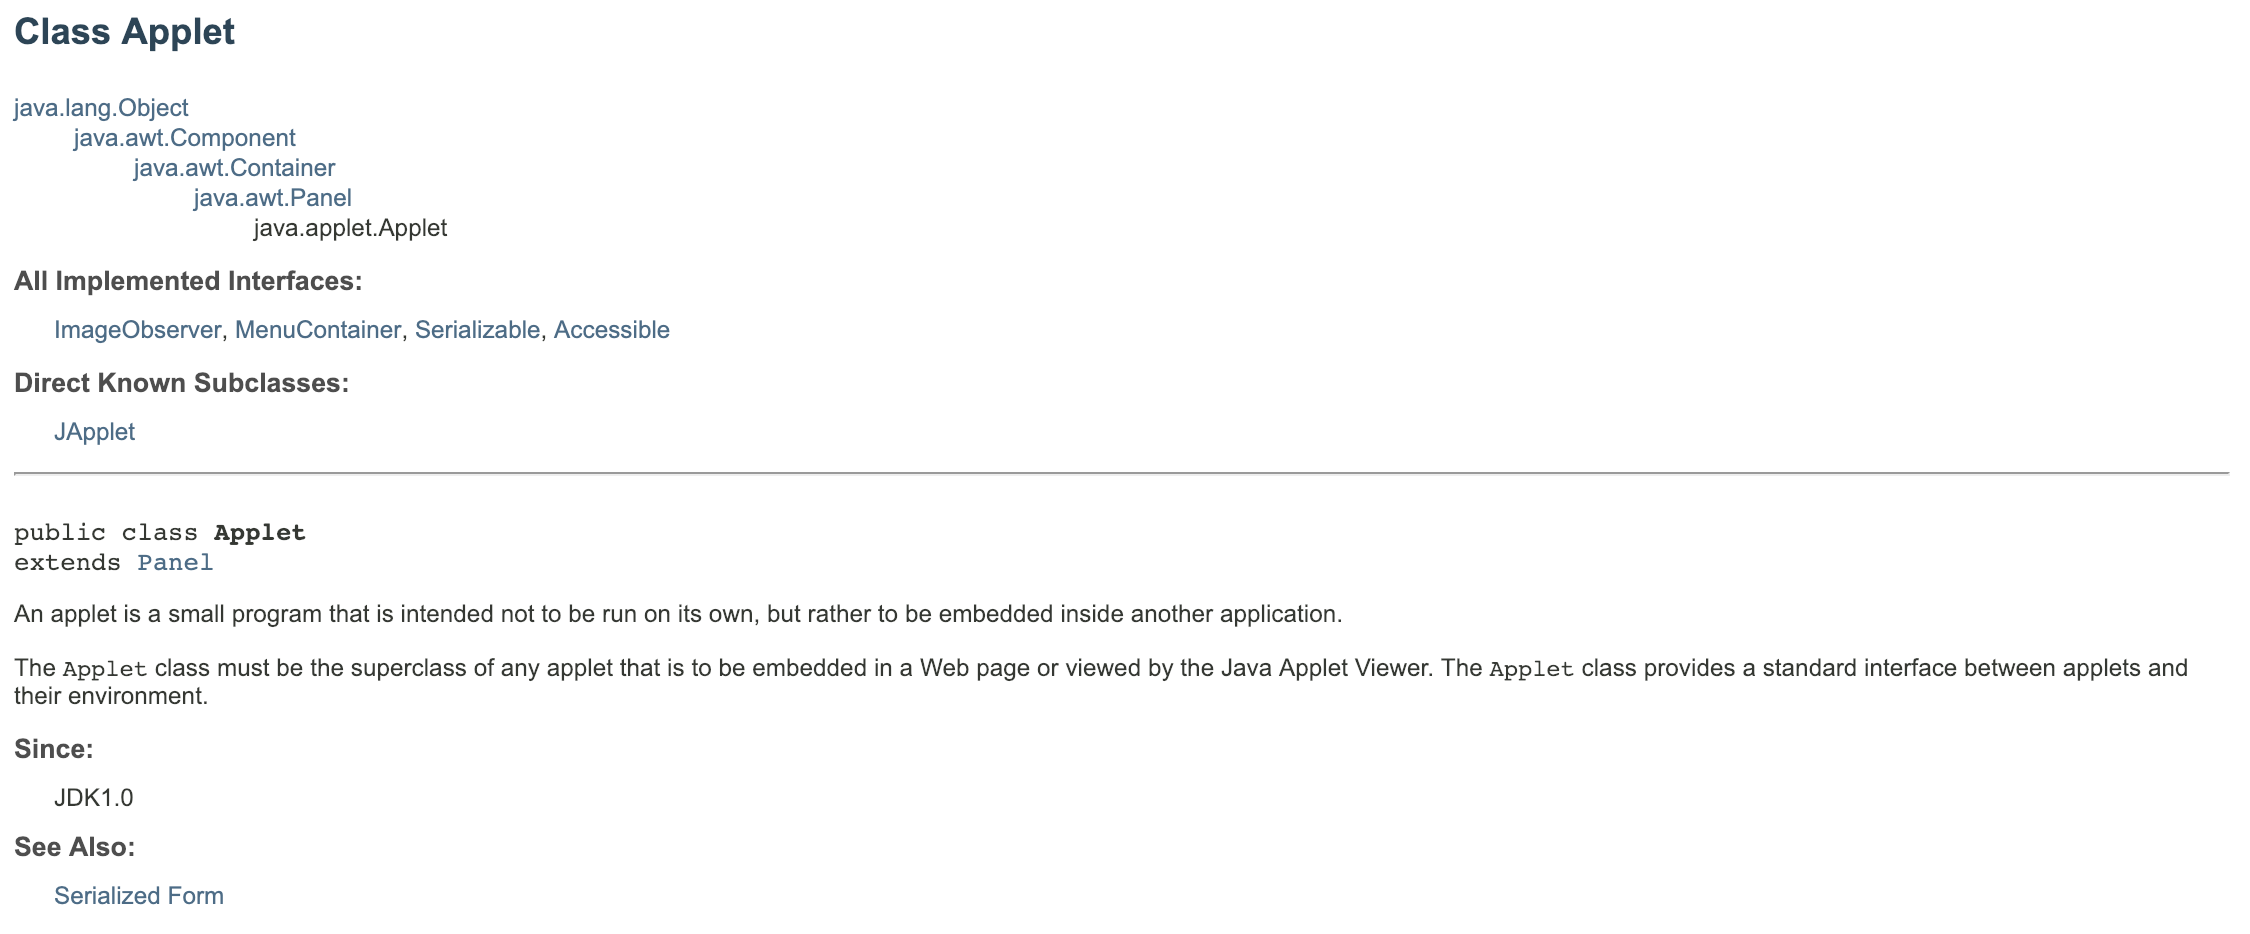
\includegraphics[scale=0.4]{a}  
	  \caption[Hasil dokumentasi pada kelas atau {\it interface}]{Hasil dokumentasi pada kelas atau {\it interface}} 
	  \label{fig:a} 
    \end{figure}
    Pada gambar \ref{fig:a}, {\it Javadoc} akan menghasilkan dokumentasinya berupa {\it file} HTML
    
	\item {\it Package Comment Files}\\
	Setiap {\it package} memiliki {\it file} yang berisikan komentar yang berkaitan dengan {\it package} tersebut. {\it File} tersebut terletak pada folder {\it package}. Contohnya {\it java/applet/package.html}, kemudian {\it Javadoc} akan menggabungkan dokumentasi tersebut menjadi sebuah ringkasan dari {\it package} yang ada. 
	Terdapat 2 cara penulisan yaitu dengan sebuah {\it file} package.html pada listing \ref{package} atau sebuah {\it file} package-info.java pada listing \ref{package-info}.
	\begin{lstlisting}[language=Html, caption={\it File package.html}, label={package}]
	<html>
	<body>
	Provides the classes necessary to create an applet and the classes
	an applet uses to communicate with its applet context.
	
	@since 1.0
	@see java.awt
	</body>
	</html>
	\end{lstlisting}
	
	\begin{lstlisting}[language=Java, caption={\it File package-info.java}, label={package-info}]
	/**
	 * Provides the classes necessary to create an applet
	 * and the classes an applet uses to communicate
	 * with its applet context.
	 *
	 * @since 1.0
	 * @see java.awt
	 */
	 package java.lang.applet;
	\end{lstlisting}
	Ketika {\it Javadoc} memproses {\it package} tersebut, {\it Javadoc} akan melakukan beberapa langkah yaitu sebagai berikut:
	\begin{enumerate}
		\item Menyalin informasi untuk diproses. Jika {\it file} berupa HTML maka pada bagian {\it <body>} hingga {\it </body>} akan disalin.
		\item Memproses semua {\it tag} yang ada.
		\item Memasukkan teks yang sudah diproses tersebut pada bagian bawah halaman dokumentasi yang dihasilkan.
		\item Menyalin kalimat pertama pada {\it package} tersebut pada bagian atas halaman dokumentasi.
	\end{enumerate}
	\begin{figure}[H]
	  \centering  
	  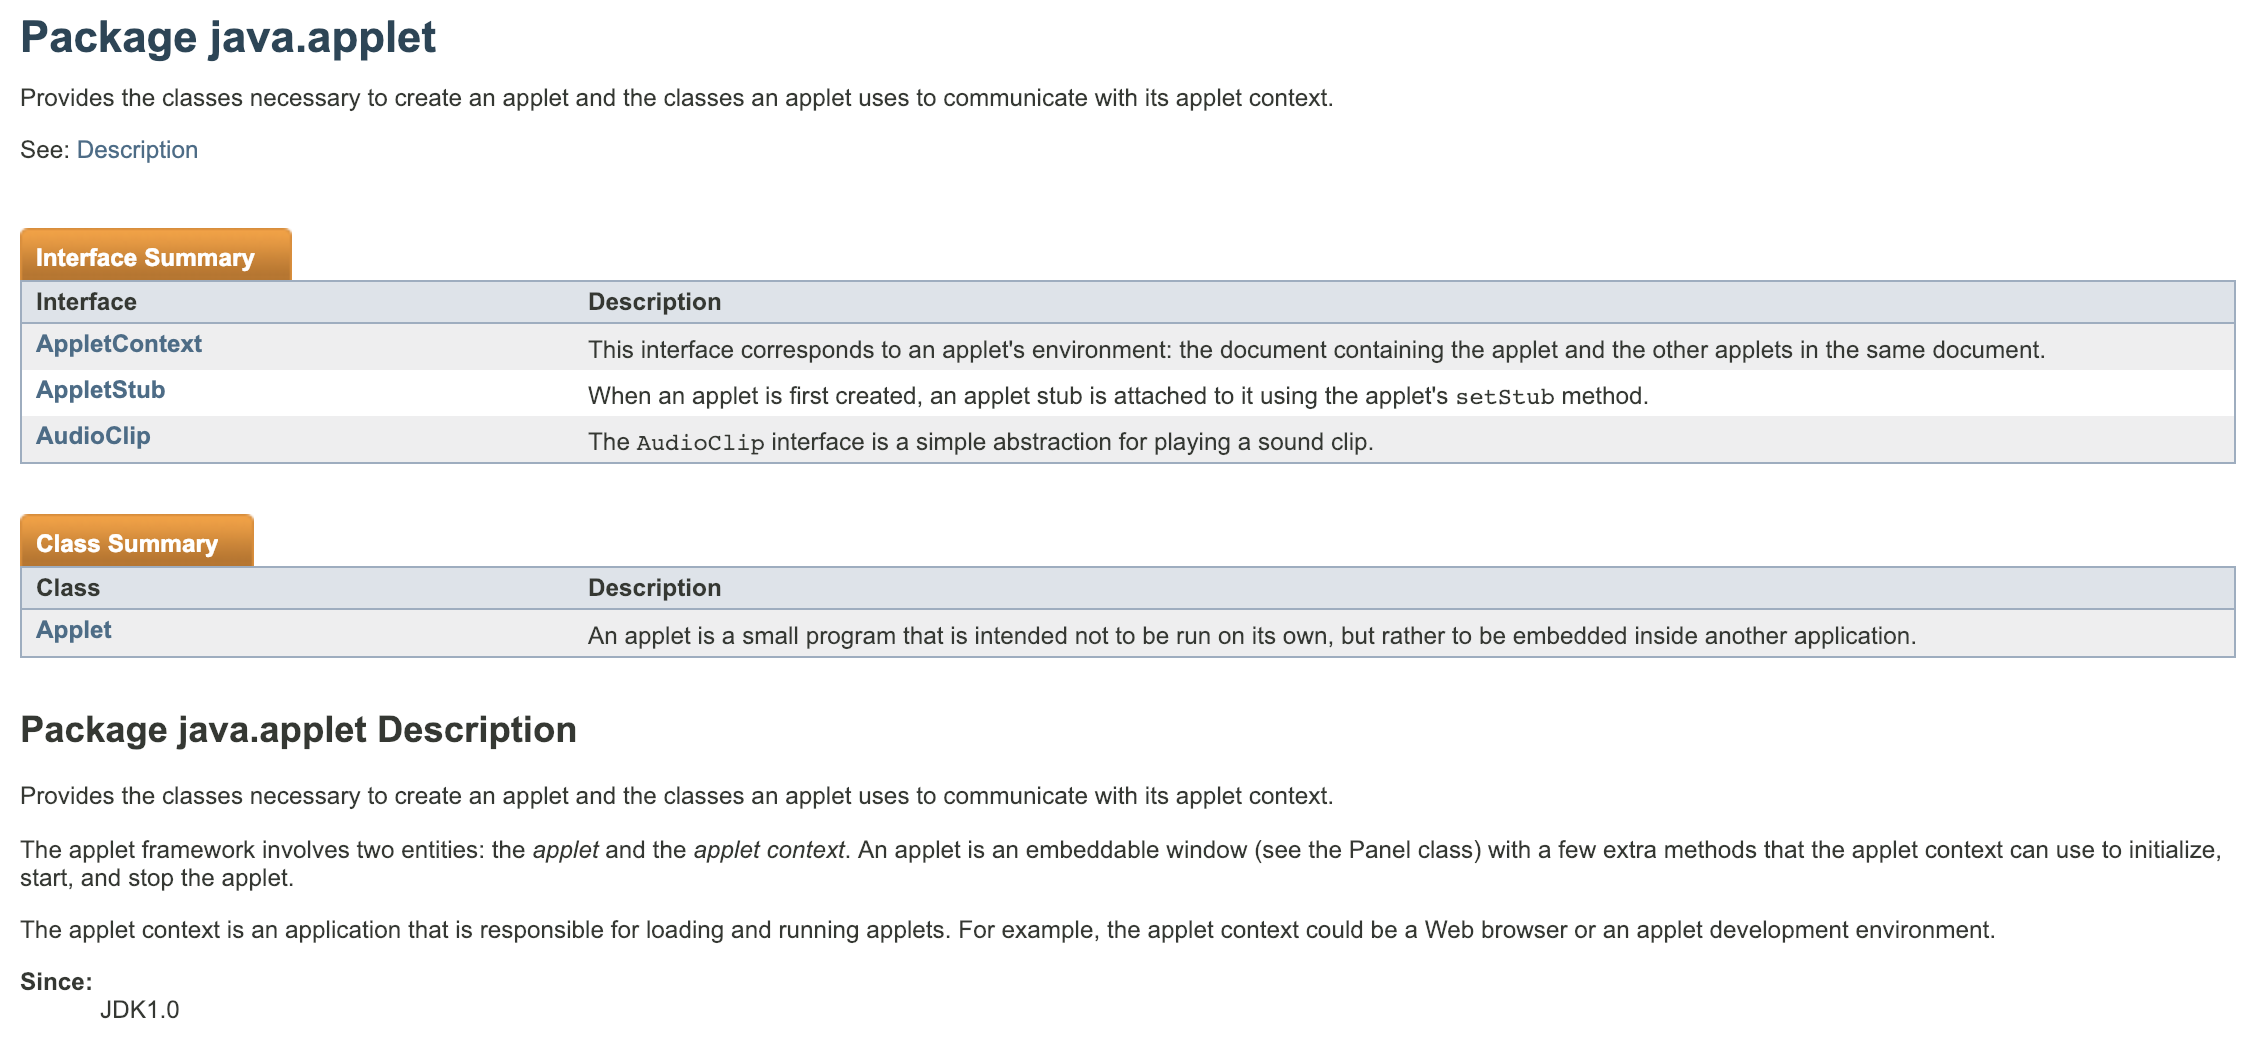
\includegraphics[scale=0.4]{b}
	  \caption[Hasil dokumentasi pada dari {\it package}]{Hasil dokumentasi pada dari {\it package}}
	  \label{fig:b} 
    \end{figure}
    Pada gambar \ref{fig:b} adalah hasil {\it Javadoc} mendokumentasikan setiap {\it package}
	\item {\it Overview Comment Files}\\
	Setiap aplikasi atau sekumpulan {\it package} yang akan didokumentasikan akan memiliki dokumentasi {\it overview}. Dokumentasi tersebut dapat dibuat lebih dari 1, jika pada saat pembuatan perangkat lunak menggunakan sekumpulan {\it package} yang berbeda.
	Untuk membuat sebuah dokumentasi ini, perlu membuat sebuah {\it file} HTML yang umumnya bernama {\it overview.html} yang diletakkan pada bagian paling atas sebuah {\it source code} yang dibuat. {\it Javadoc} akan melakukan beberapa langkah yaitu sebagai berikut:
	\begin{enumerate}
		\item Menyalin informasi untuk diproses.
		\item Memproses semua {\it tag} yang ada.
		\item Memasukan teks yang sudah diproses tersebut pada bagian bawah halaman dokumentasi yang dihasilkan.
		\item Menyalin kalimat pertama pada {\it package} tersebut pada bagian atas halaman dokumentasi.
	\end{enumerate}
	Hasil dari dokumentasi {\it overview} terdapat pada gambar \ref{fig:c}.
	\begin{figure}[H]
	  \centering  
	  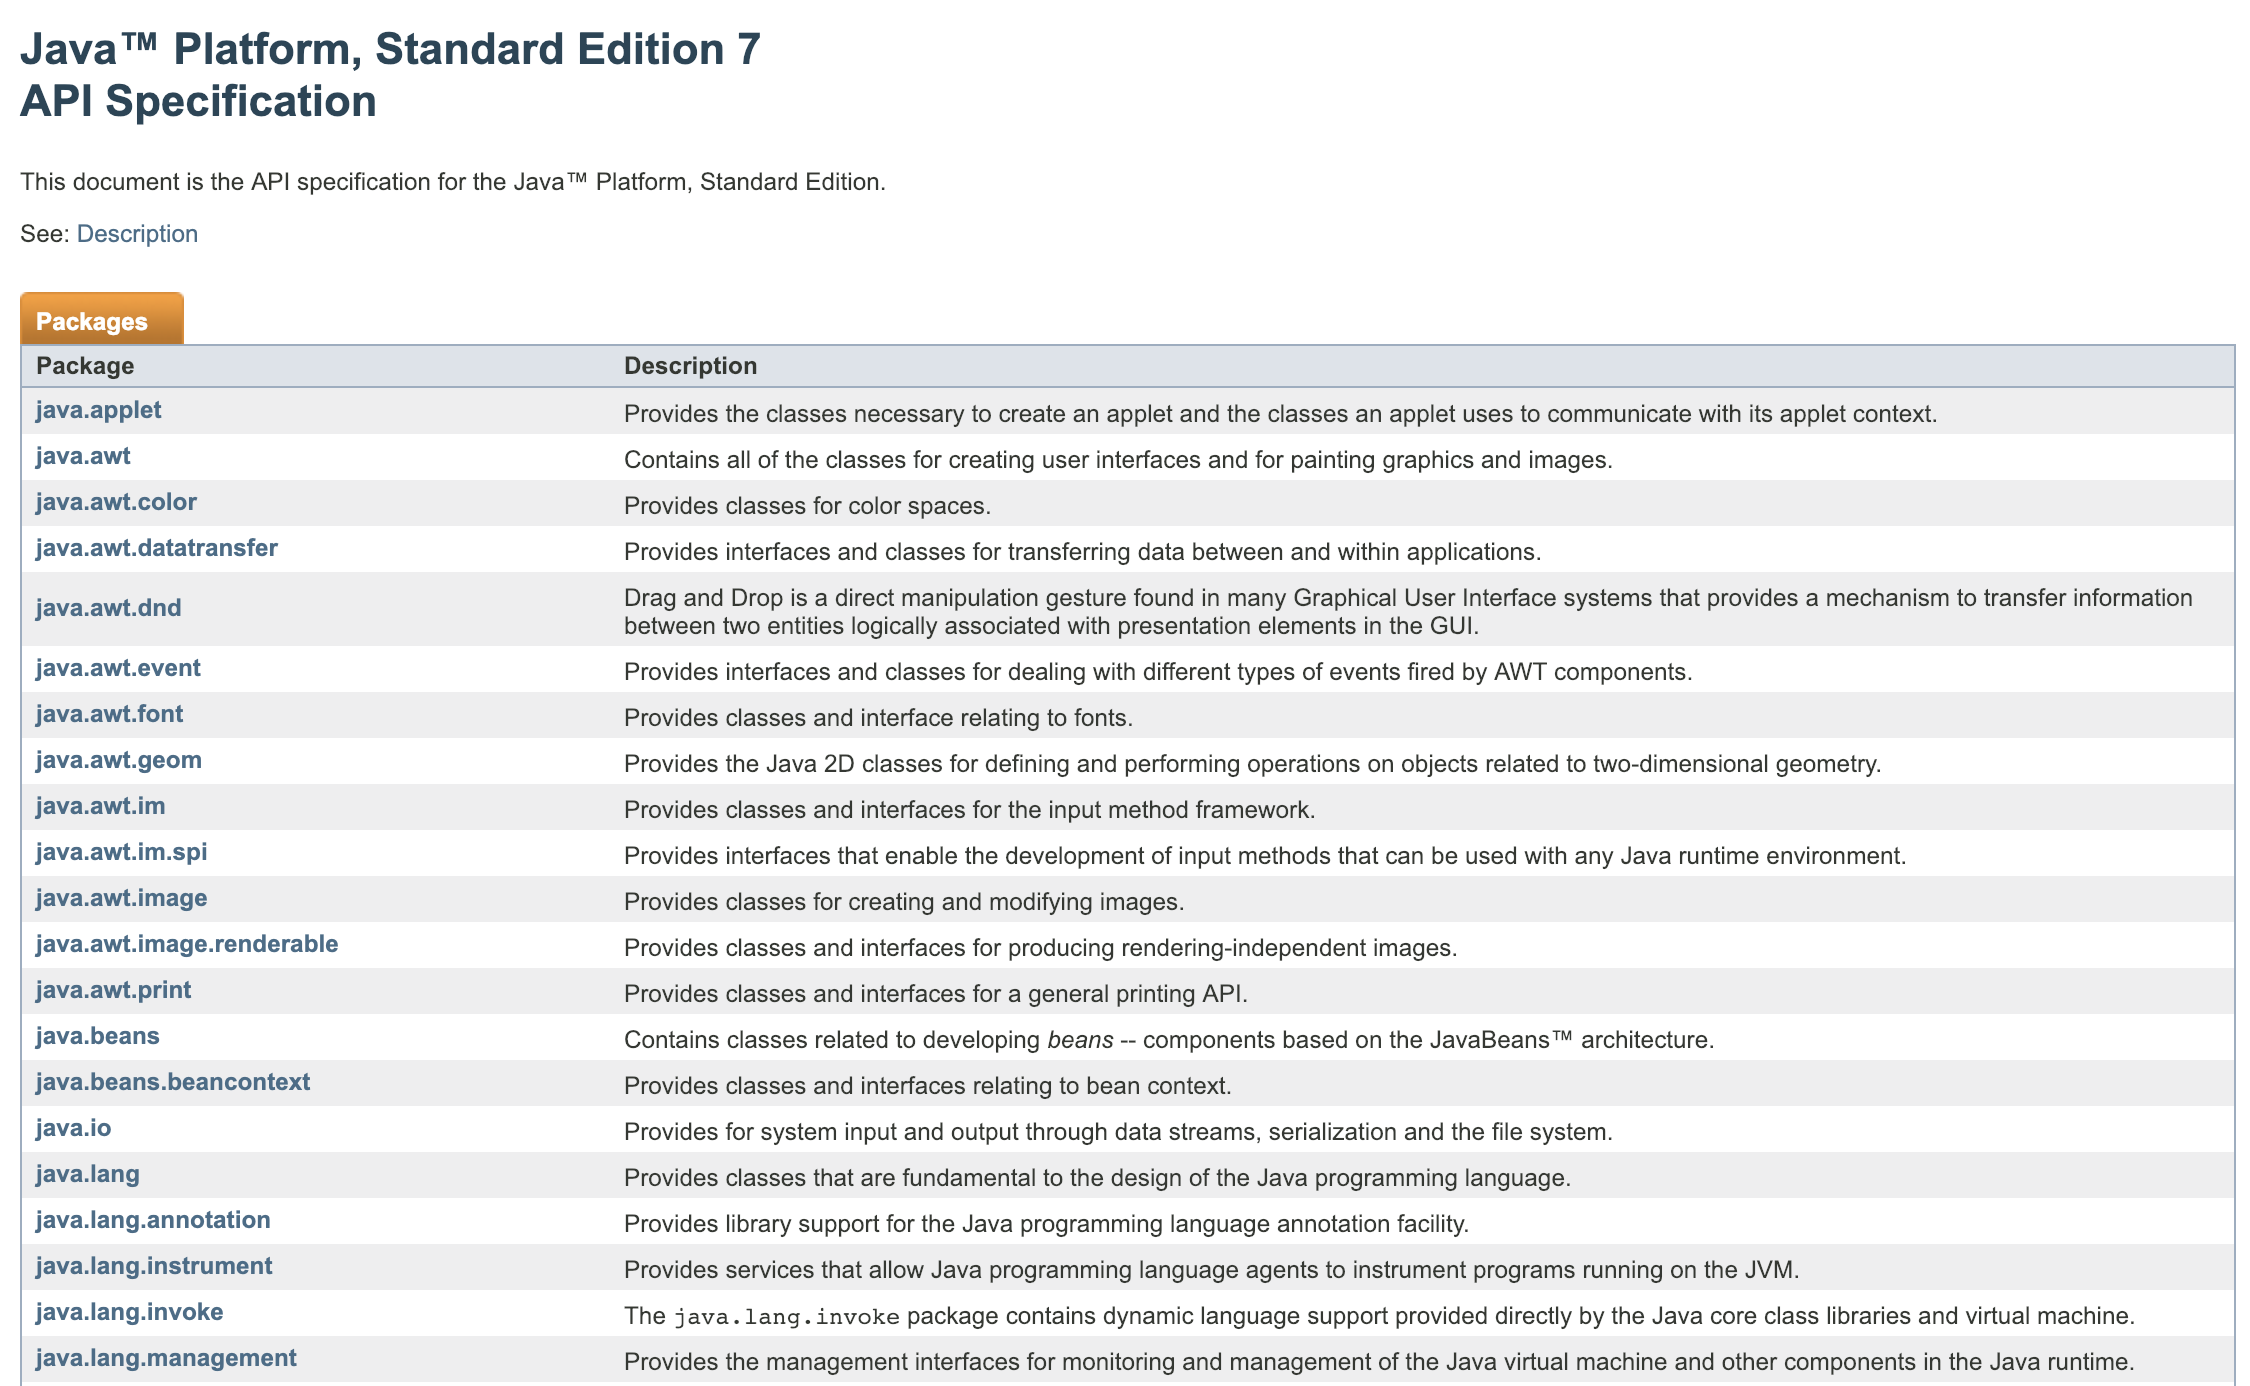
\includegraphics[scale=0.4]{c}
	  \caption[Hasil dokumentasi pada dari {\it overview}]{Hasil dokumentasi pada dari {\it overview}}
	  \label{fig:c} 
    \end{figure}
	\item {\it Miscellaneous Unprocessed Files}\\
	{\it Javadoc} dapat memproses berbagai macam format {\it file}. {\it File} tersebut dapat berupa sebuah {\it graphic files}, {\it Java source (.java)} dan {\it class (.class)} dan sebuah {\it file} HTML.
	Untuk memproses {\it file} tersebut, perlu membuat sebuah folder bernama {\it doc-files} yang diletakkan pada {\it package} tertentu lalu {\it file-file} tersebut dapat diakses dengan menggunakan lokasi direktori yang menyimpan {\it file} tersebut. Sebagai contoh jika terdapat sebuah gambar {\tt myimage.jpg} yang terletak dalam folder {\it doc-files} maka cara mengaksesnya adalah dengan menulis {\tt doc-files/myimage.jpg}.
\end{itemize}

\subsection{\textit{Generated Files}}
\label{sec:generated-files}
{\it Javadoc} memiliki sebuah {\it doclet} bawaan yang disebut dengan standar {\it doclet}. Standar {\it doclet} akan menghasilkan dokumentasi dengan format HTML. Terdapat 3 grup yaitu {\it Basic Content Pages}, {\it Cross-Reference Pages} dan {\it Support Files}. Setiap grup tersebut memiliki kriterianya sendiri, ketiga grup tersebut adalah sebagai berikut:
\begin{itemize}
	\item {\it Basic Content Pages}
	\begin{itemize}
		\item Sebuah halaman kelas atau {\it interface} ({\it classname.html}) untuk masing-masing kelas atau {\it interface} yang akan didokumentasikan.
		\item Sebuah halaman {\it package} ({\it package-summary.html}) untuk masing-masing {\it package} yang akan didokumentasikan.
		\item Sebuah halaman {\it overview} ({\it overview-summary.html}) untuk keseluruhan sekumpulan {\it package}. Halaman ini adalah halaman utama yang dihasilkan.
	\end{itemize}
	\item {\it Cross-Reference Pages}
	\begin{itemize}
		\item Sebuah halaman hirarki untuk keseluruhan {\it package} ({\it overview-tree.html}).
		\item Sebuah halaman hirarki untuk setiap {\it package} ({\it package-tree.html}).
		\item Sebuah halaman {\it "use"} ({\it package-use.html}) yang berisikan {\it package}, {\it classes}, {\it methods}, {\it constructors} atau {\it interface}. Jika diberikan sebuah kelas bernama A, maka halaman tersebut akan berisikan {\it subclasses} dari A, {\it methods} yang memiliki {\it return} A dan {\it methods} atau {\it constructors} dengan parameter bertipe A.
		\item Sebuah halaman {\it deprecated API} ({\it deprecated-list.html}). Halaman ini adalah halaman dari sekumpulan kelas atau {\it interface} yang tidak direkomendasikan untuk digunakan.
		\item Sebuah halaman sekumpulan nilai {\it constant} ({\it constant-values.html}) untuk sekumpulan nilai {\it static}.
		\item Sebuah halaman {\it serialized form} ({\it serialized-form.html}).
		\item Sebuah halaman {\it index} ({\it index-*.html}).
	\end{itemize}
	\item {\it Support Files}
	\begin{itemize}
		\item Sebuah halaman bantuan ({\it help-doc.html}).
		\item Sebuah halaman {\it index} ({\it index.html}) yang membuat sebuah HTML {\it frames}.
		\item Seberapa {\it frame file} ({\it *-frame.html}) yang berisi sekumpulan {\it packages}, kelas dan {\it interface} dan digunakan pada saat HTML {\it frames} ditampilkan.
		\item Sebuah {\it file} teks {\it package list} ({\it package-list}).
		\item Sebuah {\it style sheet file} ({\it stylesheet.css}) untuk mengontrol warna, jenis {\it font}, ukuran {\it font} dan posisi dari halaman yang dihasilkan.
		\item Sebuah {\it doc-files} yang berisikan gambar dan beberapa contoh {\it file Java}.
	\end{itemize}
\end{itemize}
{\it Javadoc} akan menghasilkan 2 atau 3 HTML {\it frame}.
	\begin{figure}[H]
	  \centering  
	  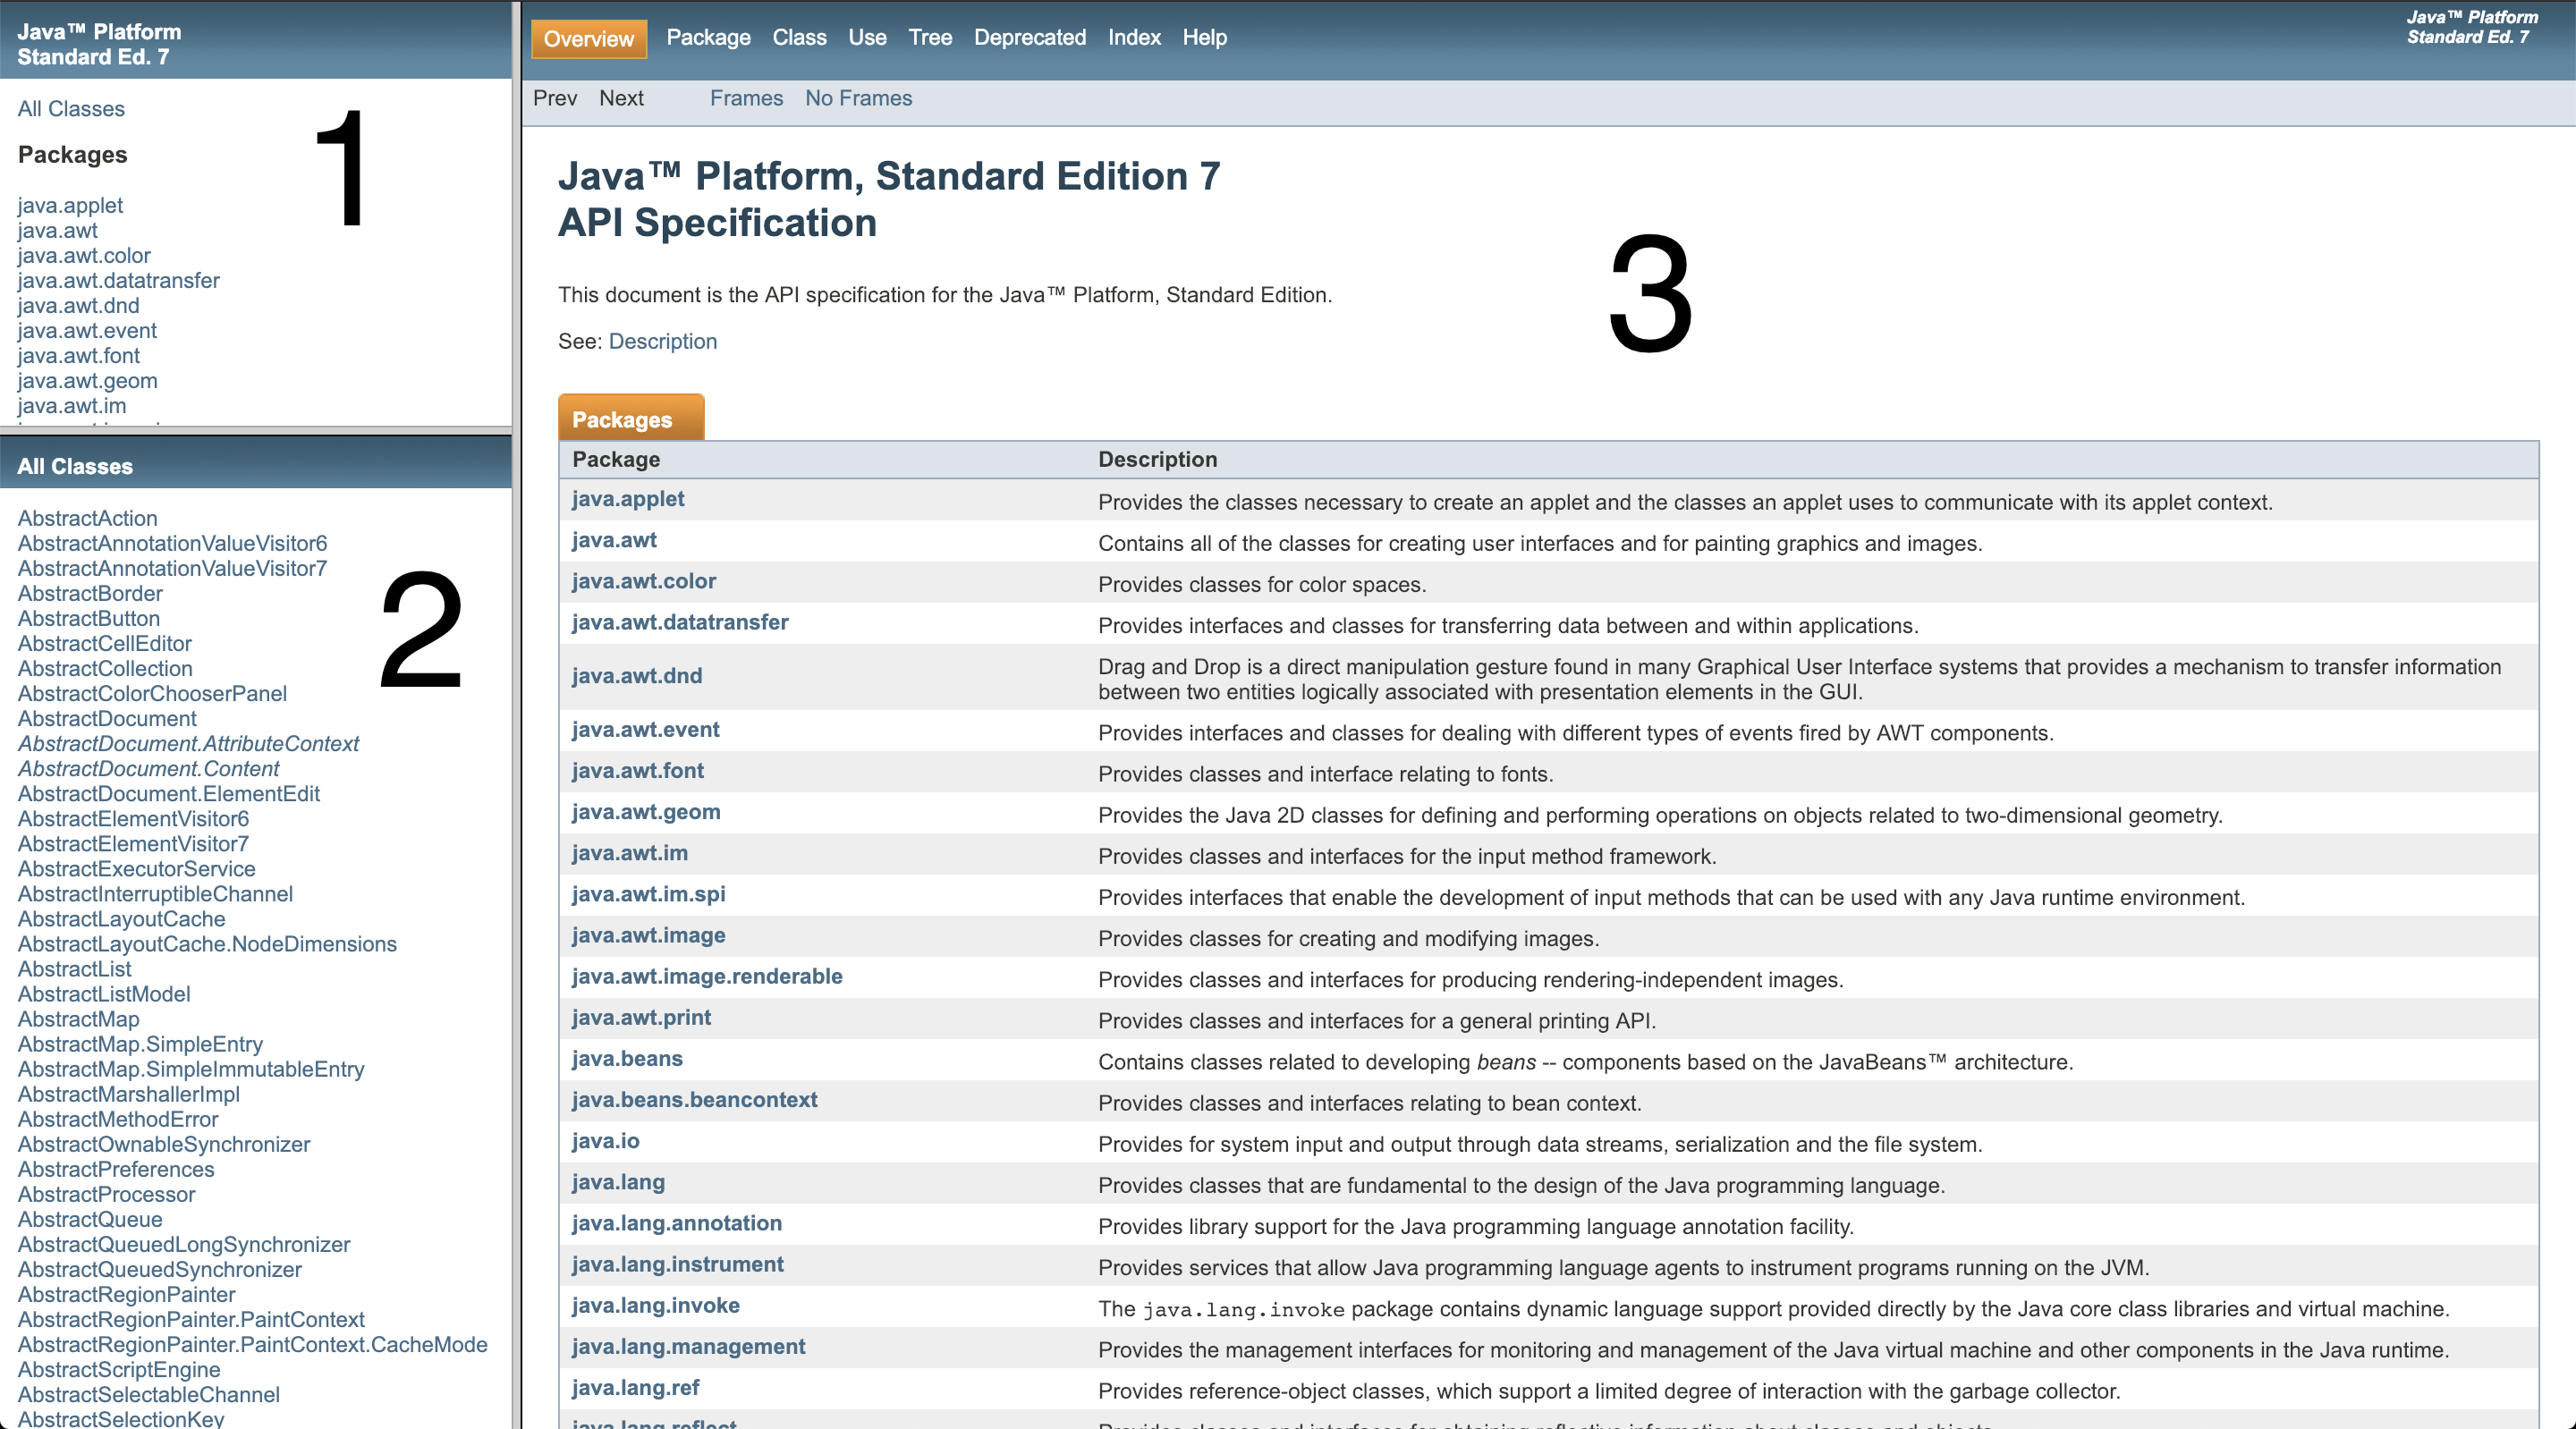
\includegraphics[scale=0.3]{d}
	  \caption[Frame pada hasil dokumentasi]{Frame pada hasil dokumentasi}
	  \label{fig:d} 
    \end{figure}
    Pada gambar \ref{fig:d} terdapat 3 buat frame. {\it Frame} pada HTML dapat disebut sebagai {\it section}. {\it Javadoc} akan membuat minimum {\it frame} yang dibutuhkan. Jika hanya terdapat 1 {\it package}, maka {\it Javadoc} akan membuat 1 {\it frame} yang berisi dari sekumpulan kelas pada {\it package} tersebut yaitu {\it frame} 3. Jika terdapat lebih dari 2 {\it package}, maka {\it Javadoc} akan membuat 3 {\it frame} dari sekumpulan {\it package} yaitu {\it frame} 1, 2 dan 3. 
Jika kelas yang digunakan adalah {\it java.applet.Applet} dan semua dokumentasi yang dihasilkan akan berada pada folder yang bernama {\it apidocs}, struktur {\it file} yang dihasilkan adalah sebagai berikut:
\begin{lstlisting}[caption=Struktur {\it file} yang dihasilkan]
	apidocs						  			  		    Top directory
		index.html											  Initial page that sets up HTML frames
	* overview-summary.html 					  Lists all packages with first sentences summaries
		overview-tree.html							  Lists class hierarchy for all packages
		deprecated-list.html              Lists deprecated API for all packages
   		constant-values.html            Lists values of static fields for all packages
   		serialized-form.html            Lists serialized form for all packages
   * overview-frame.html              Lists all packages, used in upper-left frame
   		allclasses-frame.html           Lists all classes for all packages, used in
   																		lower-left frame
   		help-doc.html                   Lists user help for how these pages are organized
   		index-all.html                  Default index created without -splitindex option
   		index-files                     Directory created with -splitindex option
       		index-<number>.html         Index files created with -splitindex option
   		package-list                    Lists package names, used only for 
   																		resolving external refs
   		stylesheet.css                  HTML style sheet for defining fonts, colors and
   																		positions
   		java                            Package directory
       		applet                      Subpackage directory
            	Applet.html             Page for Applet class
            	AppletContext.html      Page for AppletContext interface
            	AppletStub.html         Page for AppletStub interface
            	AudioClip.html          Page for AudioClip interface
          * package-summary.html    	Lists classes with first sentence summaries
          														for this package
          * package-frame.html      	Lists classes in this package, used in
          														lower left-hand frame
          * package-tree.html       	Lists class hierarchy for this package
            package-use             	Lists where this package is used
            	doc-files               Directory holding image and example files
            	class-use               Directory holding pages API is used
                	Applet.html         Page for uses of Applet class
                	AppletContext.html  Page for uses of AppletContext interface
                	AppletStub.html     Page for uses of AppletStub interface
                	AudioClip.html      Page for uses of AudioClip interface
   		src-html                        Source code directory
       		java                        Package directory
           		applet                  Subpackage directory
                	Applet.html         Page for Applet source code
                	AppletContext.html  Page for AppletContext source code
                	AppletStub.html     Page for AppletStub source code
                	AudioClip.html      Page for AudioClip source code
\end{lstlisting}
\section{Doclet}
\label{sec:doclet}
{\it Doclet} yang terdapat pada {\it Javadoc} dapat digunakan untuk menghasilkan sebuah {\it output Javadoc} yang dapat disesuaikan. Standar {\it doclet} yang dihasilkan oleh {\it Javadoc} adalah dokumentasi dengan format HTML. Selain menghasilkan {\it output} yang dapat disesuaikan, {\it Doclet} juga dapat mengambil informasi secara spesifik~\cite{doclet:02:doclet}.

\subsection{\textit{Interface-interface} pada Doclet}
\label{sec:interface-doclet}
Berikut adalah beberapa {\it interface} yang terdapat pada {\it Doclet}:
\begin{itemize}
	\item {\tt RootDoc}\\
	sebuah {\it interface} yang menjadi parameter masukan sebuah {\it doclet} dari perangkat lunak yang dibuat. Dari {\it root} tersebut semua informasi dapat diambil. {\it Method-method} yang digunakan adalah sebagai berikut:
	\begin{itemize}
		\item {\tt classes()}\\
		{\it Method} ini akan mengembalikan sejumlah kelas dan {\it interface} pada {\it package}.
	\end{itemize}
	\item {\tt ClassDoc}\\
	sebuah {\it interface} yang menyatakan informasi dari sebuah kelas. Informasi tersebut dapat berupa nama kelas, nama {\it method} dan {\it tag}. {\it Method-method} yang digunakan adalah sebagai berikut:
	\begin{itemize}
		\item {\tt name()}\\
		{\it Method} ini akan mengembalikan sebuah nama kelas atau {\it interface} pada {\it package}.
		\item {\tt commentText()}\\
		{\it Method} ini akan mengembalikan sebuah informasi dari deskripsi kelas.
		\item {\tt methods()}\\
		{\it Method} ini akan mengembalikan sebuah {\it array of methods}.
	\end{itemize}
	\item {\tt MethodDoc}\\
	sebuah {\it interface} yang menyatakan informasi dari sebuah {\it method}. {\it Method-method} yang digunakan adalah sebagai berikut:
	\begin{itemize}
		\item {\tt name()}\\
		{\it Method} ini akan mengembalikan sebuah nama {\it method}.
		\item {\tt modifiers()}\\
		{\it Method} ini akan mengembalikan sebuah {\it access modifier} dari sebuah {\it method}.
		\item {\tt returnType()}\\
		{\it Method} ini akan mengembalikan sebuah {\it return type} dari sebuah {\it method}.
		\item {\tt flatSignature()}\\
		{\it Method} ini akan mengembalikan {\it signature} dari sebuah {\it method}. Jika terdapat {\it Method} dengan parameter (String x, int y), maka akan mengembalikan (String, int).
	\end{itemize}
	\item {\tt ParamTag}\\
	sebuah {\it interface} yang menyatakan informasi dari sebuah {\it Tag} parameter. {\it Method-method} yang digunakan adalah sebagai berikut:
	\begin{itemize}
		\item {\tt name()}\\
		{\it Method} ini akan mengembalikan sebuah {\it tag @param}.
		\item {\tt parameterName()}\\
		{\it Method} ini akan mengembalikan sebuah nama parameter dari sebuah {\it method}.
		\item {\tt parameterComment()}\\
		{\it Method} ini akan mengembalikan sebuah deskripsi dari parameter yang terdapat pada {\it method}.
	\end{itemize}
\end{itemize}

\subsection{Penggunaan Doclet}
\label{sec:penggunaan-doclet}
Doclet dapat menghasilkan sebuah {\it output Javadoc} yang dapat disesuaikan. Penggunaan {\it Doclet} API dapat mengambil bermacam-macam informasi seperti nama kelas, nama {\it method}, deskripsi singkat untuk sebuah parameter dari sebuah {\it method} hingga {\it return type} dari {\it method}.

Berikut adalah langkah-langkah dasar untuk membuat dan menggunakan {\it doclet}:
\begin{enumerate}
	\item Membuat sebuah kelas {\it Java} yang akan menjadi {\it doclet}. Kelas {\it Java} tersebut harus ditambahkan {\it package} {\tt com.sun.javadoc.*} untuk menggunakan {\it doclet} API.
	\item Kelas tersebut harus diawali dengan sebuah {\it method} {\tt public static boolean start} yang memiliki parameter {\tt RootDoc}.
	\item {\it Compile} doclet tersebut dengan menggunakan {\it compiler Java} yaitu {\tt javac} yang dapat dilakukan melalui {\it Terminal} pada Linux/Mac atau {\it Command Prompt} pada Windows.
	\item Jalankan perintah {\it Javadoc} menggunakan {\it option} {\tt -doclet <class>} untuk menghasilkan {\it output} yang telah disesuaikan, dimana {\tt <class>} adalah kelas {\it doclet} yang sudah di-{\it compile} pada langkah ketiga. Jika tidak menggunakan {\it option} {\tt -doclet} maka {\it Javadoc} akan menghasilkan {\it output} standar yaitu berupa {\it file} HTML.
\end{enumerate}

Kelas-kelas yang dimiliki oleh {\it doclet} API terdapat pada direktori {\tt lib\string\tools.jar}. {\it Doclet} yang sudah dibuat harus di-{\it compile} menggunakan {\it file} {\tt tools.jar} dan menambahkan {\it option} {\tt -classpath} setelah {\it command} {\tt javac}. 

{\it Package} {\tt com.sun.javadoc.*} terdiri dari {\it interface} yang mendefinisikan {\it doclet} API. {\tt tools.jar} berisikan {\it interface} tersebut.

\begin{lstlisting}[language=Java, caption=kelas ListClass.java, label={program-doclet}]
	import com.sun.javadoc.*;

	public class ListClass {
		public static boolean start(RootDoc doc) {
			ClassDoc[] classes = doc.classes();
			for(int i=0, i < classes.length; i++) {
				System.out.println(classes[i]);
			}
			return true;
		}
	}
\end{lstlisting}
Potongan {\it program} pada Listing \ref{program-doclet} adalah sebuah perogram sederhana menggunakan {\it doclet} untuk menampilkan nama dari kelas yang dijadikan sebagai masukan. {\it Method} {\tt public static boolean start} memiliki parameter {\tt RootDoc doc} yang akan menampung masukan dari sekumpulan {\it file Java} yang akan diproses lalu sekumpulan {\it file} tersebut akan ditampung pada {\tt ClassDoc[] classes} sebagai {\tt array} kemudian {\it array of classes} akan dijalankan sebanyak panjang {\it array} tersebut.

\section{\LaTeX}
\label{sec:latex}
\LaTeX\ adalah sebuah bahasa {\it markup} untuk sistem penulisan dokumen yang dikembangkan oleh Leslie B. Lamport dan dirilis pada tahun 1985~\cite{latex:03:latex}.  Bahasa {\it markup} adalah sebuah bahasa yang menganotasikan dokumen dengan cara menambahkan sintaks tertentu agar dapat dibedakan.  \LaTeX\ Memiliki filosofi WYMIWYG ({\it What you Mean Is What You Get}) yang berarti sesuatu yang ditulis akan berdasarkan arti dari hal tersebut. Oleh karena itu, untuk menambahkan suatu perintah pada dokumen yang sedang ditulis perlu menambahkan suatu {\it command}. {\it Command} adalah kata spesial yang menentukan suatu sifat pada \LaTeX. Hampir semua {\it command} pada \LaTeX\ selalu diawali dengan tanda '$\backslash$' dan beberapa {\it command} memiliki {\it parameter}. {\it Parameter} diawali dengan tanda kurung kurawal buka dan diakhiri dengan kurung kurawal tutup (\{...\}). File \LaTeX\ memiliki ekstensi .tex. Pada saat membuat sebuah {\it project} \LaTeX\ hanya perlu menuliskan {\it command} \texttt{\string\documentclass[option]\{class\}} 1 kali.

Untuk menulis dokumen pada \LaTeX\ dibutuhkan beberapa {\it command} yang wajib ada dalam sebuah dokumen, yaitu:
\begin{enumerate}
	\item \texttt{\string\documentclass[option]\{class\}}\\
	Digunakan untuk menentukan jenis dokumen yang {\it layout} dokumen. Bagian {\it option} dapat dikosongkan atau dapat digunakan untuk menyimpan pilihan pengaturan {\it layouting}. Pada Bagian kelas digunakan untuk menentukan tipe dokumen yang akan dibuat. {\it Command} ini hanya perlu ditulis 1 kali dalam sebuah dokumen.
	\item \texttt{\string\maketitle}\\
	Digunakan untuk menampilkan halaman judul. Biasanya halaman judul akan memuat judul dokumen, nama pengarang dan tanggal pembuatan dokumen. Judul dokumen, nama pengarang dan tanggal pembuatan dapat ditampilkan dengan menambahkan perintah \texttt{\string\title\{judul\}}, \texttt{\string\author\{nama\}} dan \texttt{\string\date\{tanggal\}}.
	\item \texttt{\string\begin\{document\}}\dots\texttt{\string\end\{document\}}\\
	Digunakan untuk mengawali dan mengakhiri sebuah dokumen.
	\item \texttt{\string\section\{section\}}\\
	Digunakan untuk menampilkan subbab sebuah dokumen.
	\item \texttt{\string\texttt\{text\}}\\
	Digunakan untuk menampilkan tulisan {\it monospaced}.
	\item \texttt{\string\textbf\{text\}}\\
	Digunakan untuk menampilkan tulisan tebal.
	\item \texttt{\string\begin\{enumerate\}}\dots\texttt{\string\end\{enumerate\}}\\
	Digunakan untuk menampilkan {\it ordered list}. {\it List} ini akan menampilkan angka yang terurut. Di dalam {\it list} ini terdapat {\it command} \texttt{\string\item} untuk menambahkan isi dari {\it list} tersebut.
	\item \texttt{\string\begin\{itemize\}}\dots\texttt{\string\end\{itemize\}}\\
	Digunakan untuk menampilkan {\it unordered list}. {\it List} ini akan menampilkan {\it bullet}. Di dalam {\it list} ini terdapat {\it command} \texttt{\string\item} untuk menambahkan isi dari {\it list} tersebut.
\end{enumerate}

\section{\textit{Syntax Java}}
\label{sec:syntax-java}

Agar dokumentasi yang dihasilkan oleh {\it Javadoc} menghasilkan hasil yang baik dibutuhkan penulisan sintaks pada kode program java yang baik. Berikut beberapa aturan yang dapat digunakan.

\begin{enumerate}
  \item \textbf{Kelas}\\
  Untuk penamaan kelas harus ditulis dengan menggunakan aturan {\it PascalCase}. {\it PascalCase} adalah aturan umum pada penulisan sebuah kode program dengan cara setiap kata diawali dengan huruf besar atau kapital. Jika ingin membuat sebuah nama kelas {\tt myapp} maka harus ditulis seperti {\tt MyApp}. Deklarasi kelas harus ditulis {\tt <access\_modifier> class <classname>}. Pada {\it Java}, {\it Access Modifier} terbagi menjadi 3 yaitu sebagai berikut.
  \begin{enumerate}
    \item {\it public} yang dapat diakses secara global diseluruh perangkat lunak
    \item {\it private} yang tidak dapat diakses secara global diseluruh perangkat lunak
    \item {\it protected} yang hanya bisa diakses jika terdapat kelas yang menjadi turunan dari kelas tersebut
  \end{enumerate}
  Pada bagian deklarasi kelas harus terdapat komentar yang berfungsi sebagai deksripsi kelas tersebut. Komentar diletakan didalam tanda {\tt /** \dots\ */}. Berikut cara penulisan kelas yang baik dan benar.
	\begin{figure}[H]
	  \centering  
	  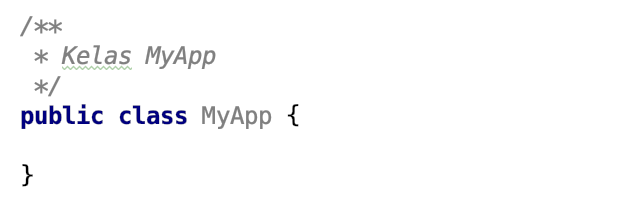
\includegraphics[scale=1]{kelas}
	  \caption[Contoh deklarasi kelas pada {\it Java}]{Contoh deklarasi kelas pada {\it Java}}
	  \label{fig:kelas} 
    \end{figure}
  \item \textbf{Atribut}\\
  Untuk penamaan atribut harus ditulis dengan menggunakan aturan {\it CamelCase}. {\it CamelCase} adalah aturan umum pada penulisan sebuah kode program dengan cara setiap kata kedua diawali dengan huruf besar atau kapital. Jika ingin membuat sebuah nama atribut {\tt islogin} maka harus ditulis seperti {\tt isLogin}. Deklarasi atribut harus ditulis {\tt <access\_modifier> <tipe\_data> <nama\_atribut>}. Terdapat beberapa tipe data yang dapat digunakan yaitu sebagai berikut.
    \begin{enumerate}
      \item {\tt byte} - untuk bilangan bulat dengan panjang $2^7 -1$.
      \item {\tt short} - untuk bilangan bulat dengan panjang $2^{15} -1$
      \item {\tt int} - untuk bilangan bulat dengan panjang $2^{31} -1$. Umumnya tipe data ini lebih sering digunakan
      \item {\tt long} - untuk bilangan bulat dengan panjang $2^{63} -1$.
      \item {\tt float} - untuk bilangan desimal dengan panjang 32-bit.
      \item {\tt double} - untuk bilangan desimal dengan panjang 64-bit.
      \item {\tt String} - sebuah objek pada {\it java} untuk kalimat.
    \end{enumerate}
  Pada bagian deklarasi atribut harus terdapat komentar yang berfungsi sebagai deksripsi atribut tersebut. Komentar diletakan didalam tanda {\tt /** \dots\ */}. Berikut cara penulisan kelas yang baik dan benar.
	\begin{figure}[H]
	  \centering  
	  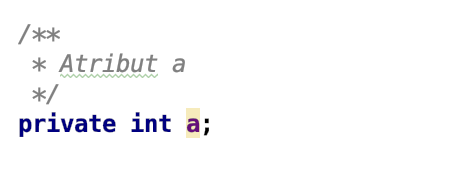
\includegraphics[scale=1]{atribut}
	  \caption[Contoh deklarasi atribut pada {\it Java}]{Contoh deklarasi atribut pada {\it Java}}
	  \label{fig:atribut} 
    \end{figure}
  \item \textbf{Method}\\
  Untuk penamaan {\it method} harus ditulis dengan menggunakan aturan {\it CamelCase}. {\it CamelCase} adalah aturan umum pada penulisan sebuah kode program dengan cara setiap kata kedua diawali dengan huruf besar atau kapital. Jika ingin membuat sebuah nama {method} {\tt getusercomments} maka harus ditulis seperti {\tt getUserComments}. Dekralasi {\it method} harus ditulis {\tt <access\_modifier> <tipe\_data\_kembalian> <atribut>(<tipe\_data\_parameter> <nama\_parameter>)}. Tipe data kembalian dan tipe data parameter sama dengan tipe data atribut.
  
  Pada bagian deklarasi kelas harus terdapat komentar yang berfungsi sebagai deksripsi kelas tersebut. Komentar diletakan didalam tanda {\tt /** \dots\ */}. Berikut cara penulisan kelas yang baik dan benar.
	\begin{figure}[H]
	  \centering  
	  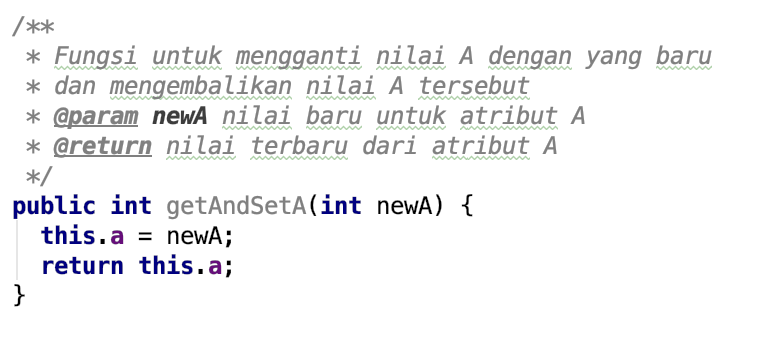
\includegraphics[scale=1]{method}
	  \caption[Contoh deklarasi {\it method} pada {\it Java}]{Contoh deklarasi {\it method} pada {\it Java}}
	  \label{fig:method} 
    \end{figure}
\end{enumerate}






